\section{Diagnosing and Mitigating Reward Hacking}

To address reward hacking, prior work identifies which training samples exploit the reward model, then removes or reweights them during optimization~\citep{liu2024rrm,beigi2026adversarial,zhang2024policy}. Following this strategy, we first diagnose which $S_{\mathrm{INIT}}$ responses the teacher assigns high advantage to, then test whether masking pathological responses or reinitializing from a cleaner distribution can prevent the collapse.




\subsection{The Teacher's Reward Signal Can Be Misaligned with Response Quality}
\label{sec:teacher_selection}

\begin{figure}[t]
    \centering
    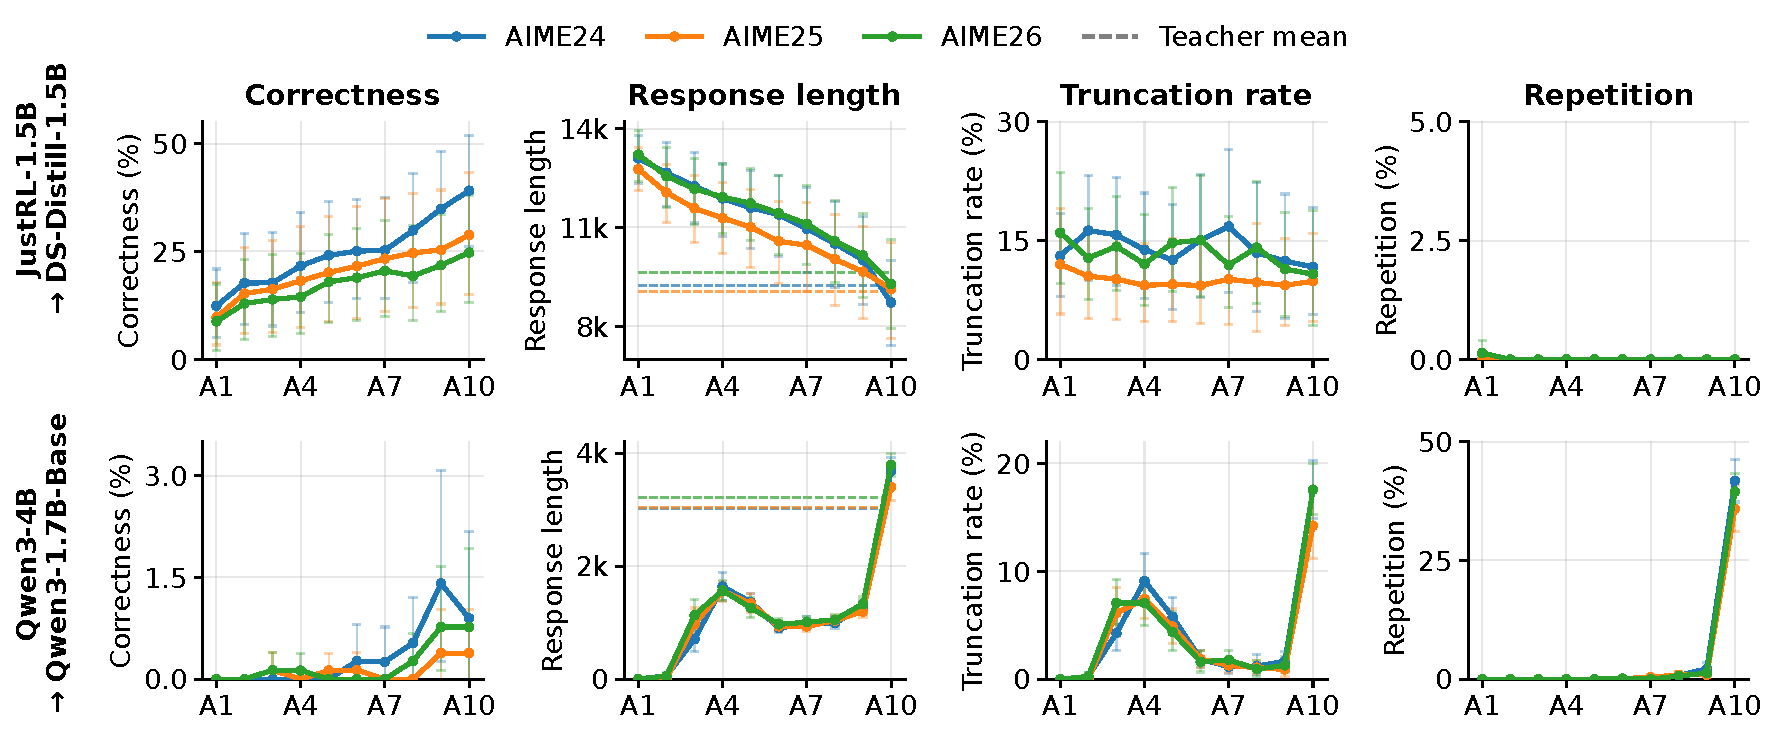
\includegraphics[width=0.95\textwidth]{figures/S4/teacher_preference_bias_matplotlib.pdf}
    \caption{
        \textbf{Teacher advantage over $S_{\mathrm{INIT}}$ responses from A1 (lowest advantage) to A10 (highest advantage).}
        The JustRL teacher (top) assigns higher advantage to correct and shorter responses; the Qwen3-4B teacher (bottom) assigns higher advantage to overlong, repetitive ones.
        Dashed lines mark the teacher's own mean length.
    }
    \label{fig:teacher_preference_bias}
\end{figure}

To characterize the responses favored by the teacher before training, we rank all sampled $S_{\mathrm{INIT}}$ responses by their mean teacher advantage and divide them into ten equally sized groups, A1--A10.
Each group contains 10\% of the responses, with A1 containing the lowest-advantage responses and A10 the highest.
Figure~\ref{fig:teacher_preference_bias} reports correctness, response length,
generation-cap hit rate, and severe-repetition rate across advantage deciles.
In the JustRL setting, teacher advantage is aligned with response quality:
correctness increases toward A10, response length decreases toward the
teacher's own average, and no severe repetition is detected.
The Qwen3-4B setting shows the opposite pattern.
The highest-advantage responses are not the most reliable ones: their correctness remains close to zero, whereas their length, truncation rate, and repetition rate increase substantially across advantage deciles.
Although these pathological
responses are rare under $S_{\mathrm{INIT}}$, the teacher assigns them high
advantage, causing OPD to amplify them during training.
We also find similar failure pattern when the teacher is replaced as Qwen3-8B and Qwen3-30B-A3B.
Appendix~\ref{app:high_advantage_examples} presents three high-advantage
$S_{\mathrm{INIT}}$ responses that exhibit excessive length and mechanical repetition.



\begin{figure}[t]
    \centering
    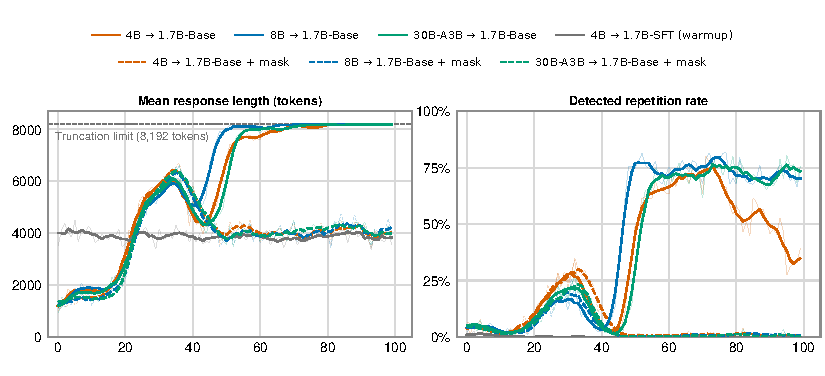
\includegraphics[width=0.95\textwidth]{S4/s4_3_candidate_pool_interventions.pdf}
    \caption{
        \textbf{Student-rollout characteristics during training.}
        All the masking settings recover from the collapse, whereas Qwen3-4B-warmup avoids it from the beginning.
    }
    \label{fig:candidate_pool_interventions}
\end{figure}


\subsection{Candidate-Pool Interventions Mitigate Reward Hacking}
\label{sec:5_2}

%
%
%
%
\begin{wraptable}{r}{0.49\textwidth}
    \centering

    \vspace{-2mm}
    \footnotesize
    \setlength{\tabcolsep}{2pt}
    \renewcommand{\arraystretch}{1.15}
    %
    \caption{
        \textbf{Masking improves average accuracy across teachers.}
        Accuracy (\%) and the four-benchmark mean; teachers are Qwen3 models,
        and Base/SFT denote Qwen3-1.7B initializations.
    }
    \label{tab:candidate_pool_interventions}
    \resizebox{\linewidth}{!}{%
    \begin{tabular}{lrrrrr}
        \toprule
        \multirow{2}{*}{\textbf{Setting}} & \textbf{AMC}
        & \multicolumn{3}{c}{\textbf{AIME}} & \multirow{2}{*}{\textbf{Avg.}} \\
        \cmidrule(lr){2-2}\cmidrule(lr){3-5}
        & \textbf{23} & \textbf{24} & \textbf{25} & \textbf{26} & \\
        \midrule
        Base (pre-OPD) & 2.41 & 1.67 & 0.00 & 1.67 & 1.44 \\
        \midrule
        4B $\rightarrow$ Base & 29.82 & 3.33 & 3.33 & 4.17 & 10.16 \\
        \quad + mask & 34.64 & 8.33 & 5.83 & 4.17 & 13.24 \\
        \midrule
        8B $\rightarrow$ Base & 28.31 & 5.00 & 3.33 & 5.00 & 10.41 \\
        \quad + mask & 32.83 & 5.00 & 2.50 & 3.33 & 10.92 \\
        \midrule
        30B-A3B $\rightarrow$ Base & 28.61 & 6.67 & 2.50 & 4.17 & 10.49 \\
        \quad + mask & 33.13 & 10.00 & 4.17 & 5.00 & 13.07 \\
        \midrule
        4B $\rightarrow$ SFT$^{\dagger}$ (warmup) & 38.86 & 9.17 & 10.00 & 7.50 & 16.38 \\
        \bottomrule
    \end{tabular}%
    }
    \vspace{-2mm}
\end{wraptable}


The preference bias discussed previously is
already visible in responses sampled from $S_{\mathrm{INIT}}$, before any OPD
update takes place.
This suggests that the collapse may depend on which
responses are supplied to the teacher for supervision. To test this hypothesis,
we intervene on the candidate pool in the Qwen3-4B setting while keeping the
teacher, training data, and optimization recipe fixed.
We consider two interventions:
(1) The \textbf{Qwen3-4B-masked setting}: masking the loss on responses that reach the generation length limit.
(2) The \textbf{Qwen3-4B-warmup setting}: changing only the student initialization, from Qwen3-1.7B-Base to an SFT-initialized student released by \citet{li2026rethinkingopd}.
Appendix~\ref{app:intervention_details} provides the training details for both interventions.
\begingroup
\renewcommand{\thefootnote}{\fnsymbol{footnote}}
\footnotetext[2]{Warmup uses the Qwen3-1.7B-SFT checkpoint released by
\citet{li2026rethinkingopd}.}
\endgroup




\textbf{Masking recovers from collapse, while warmup avoids it.}
Figure~\ref{fig:candidate_pool_interventions} shows how response length, truncation, and repetition evolve over the course of training.
The original Qwen3-4B setting eventually enters a persistent collapsed state, where responses become increasingly long, truncated, and repetitive.
For the Qwen3-4B-masked setting, the student model exhibits few abnormal behaviors in the early training phase, so its learning trajectory closely aligns with that of the original Qwen3-4B.
As the undesirable behaviors accumulate, the effect of the masking intervention becomes clear: the Qwen3-4B-masked setting recovers, while the original setting collapses.
On the other hand, the warmup setting never develops this failure mode.
Warmup has been adopted as a remedy for OPD collapse~\citep{li2026rethinkingopd}.
The SFT-initialized student rarely produces the pathological responses favored by the teacher, leaving fewer such responses for OPD to reinforce.
Together, these results suggest that the collapse is not irreversible;
it depends on whether abnormal responses continue to receive reinforcement during training.



\textbf{Both interventions improve final accuracy.}
Table~\ref{tab:candidate_pool_interventions} extends the accuracy comparison to Qwen3-8B and Qwen3-30B-A3B teachers.
Masking improves the average accuracy over AMC23 and AIME24--26 by 3.08, 0.51, and 2.58 percentage points for the 4B, 8B, and 30B-A3B teachers, respectively.
These gains are not uniform across benchmarks: with the 8B teacher, AIME24 accuracy is unchanged while AIME25 and AIME26 accuracy decrease from 3.33\% to 2.50\% and from 5.00\% to 3.33\%, respectively.
The 4B warmup setting starts from a stronger SFT student and achieves the best final average accuracy (16.38\%), exceeding the corresponding Base-initialized OPD setting by 6.22 points.
In the 4B masking setting, accuracy improves even though only approximately 10\% of the sampled responses retain nonzero loss after abnormal responses are masked.
